\documentclass[10pt,a4paper]{article}
\usepackage[T1]{fontenc}
\usepackage[utf8]{inputenc}
\usepackage{lmodern}
\usepackage[margin=21mm]{geometry}
\usepackage{microtype}
\usepackage{graphicx}
\usepackage{booktabs,tabularx,array,multirow}
\usepackage{amsmath,amssymb}
\usepackage{xcolor}
\usepackage[font=small,labelfont=bf]{caption}
\usepackage{enumitem}
\usepackage[section]{placeins}
\usepackage[hidelinks]{hyperref}
\graphicspath{{figures/}}
\setlist{nosep,leftmargin=*}
\newcolumntype{Y}{>{\raggedright\arraybackslash}X}
\newcommand{\pts}{\,pts}

\title{Hard, Fuzzy and Adaptive Temporal Eye-Tracking Gates for Entropy-Based Fuzzy EEG Classification:\\
\large An Evaluation on Real EEG and Eye-Tracking Data (ZuCo~1.0)}
\author{Soft Computing Project Report}
\date{November 2026}

\begin{document}
\maketitle

\begin{abstract}
\noindent
We re-implemented the eye-gated EEG emotion-recognition pipeline of Farhadi Sedehi et al.\ (IEEE Access, 2024). The pipeline uses wavelet-band entropy features, mRMR feature selection and a Sugeno fuzzy inference system whose rules are tuned by a genetic algorithm. An eye-tracking gate decides which EEG windows the classifier trusts. The paper's gate is a hard pupil threshold (M0). We propose and evaluate three softer gates: a fuzzy Low/Medium/High pupil gate (M1); an adaptive temporal fuzzy gate with per-participant breakpoints and smoothing over time (M2); and M1 combined with M2's temporal smoothing (M1\,+\,temporal). SEED-IV and MAHNOB-HCI require signed licences, so all models were evaluated on the free ZuCo~1.0 corpus: 12 participants, 4{,}430 sentences, simultaneous EEG and eye tracking, labelled with three-class sentence sentiment. Running the pipeline on real data exposed eight defects, all corrected identically for every model. After correction, all models perform at chance level (32--35\%; chance 33.3\%). The proposed gates lead M0 by $+0.2$ to $+0.5$ points under 5-fold cross-validation and trail it by $-0.2$ to $-0.6$ points under leave-one-subject-out validation. None of these differences is significant. A non-fuzzy logistic-regression reference on all 380 EEG features and the eye features reaches only 35\%, so on ZuCo the features carry almost no sentiment information and no gate can show a benefit. The fuzzy gates do not harm performance, and M1\,+\,temporal was the most consistent of them. A fair test of the proposed gates requires an induced-emotion dataset such as SEED-IV.
\end{abstract}

\section{Objective and models}
The project asks whether replacing the paper's hard eye-tracking threshold with softer, fuzzy gating improves EEG-based affect classification. All models share every component except the gate, which assigns a weight $w_t$ to each 1-s window $t$:
\begin{itemize}
  \item \textbf{No gate} (reference): $w_t=1$.
  \item \textbf{M0, hard gate} (paper baseline): $w_t=1$ if the window's pupil value is in the top 40\% of its trial, and 0 otherwise.
  \item \textbf{M1, fuzzy gate} (proposed): graded $w_t\in[0.1,1]$ from a three-rule Sugeno system on the pupil signal, scaled per participant.
  \item \textbf{M2, adaptive temporal fuzzy gate} (proposed): as M1, but with per-participant percentile breakpoints (\emph{adaptive}) and weights smoothed over neighbouring windows (\emph{temporal}). Two ablations isolate its parts: \emph{M2 adaptive-only} (no smoothing) and \emph{M2 causal} (smoothing over past windows only, so it can run in real time).
  \item \textbf{M1\,+\,temporal}: M1 with M2's temporal smoothing and M1's fixed breakpoints.
  \item \textbf{M1 v1} (ablation): our first M1, scaled within each trial instead of per participant (\S\ref{sec:fixes}).
\end{itemize}
Multi-band probability fusion (former M3) and its combination with M2 (former M4) were removed from the project. All gates are label-free: they use only the eye signal.

\section{Method}
\subsection{Shared pipeline}
\begin{enumerate}
  \item \textbf{Preprocessing.} 4th-order Butterworth band-pass (1--60\,Hz) and a 50\,Hz notch, applied to each continuous recording block before cutting trials (to avoid edge artefacts); then resampling to 128\,Hz.
  \item \textbf{Bands.} A 4-level db4 wavelet decomposition gives delta (0--4\,Hz), theta (4--8), alpha (8--16), beta (16--32) and gamma (32--64\,Hz).
  \item \textbf{Features.} For each non-overlapping 1-s window, band and channel we compute four entropies: SampEn ($m{=}2$), permutation entropy ($m{=}3,\tau{=}1$), symbolic dynamic entropy ($m{=}3,\tau{=}1$) and phase entropy. Each feature is z-scored within participant. The eye features per window are fixation duration (mean, SD, max), fixation rate, and pupil diameter (mean, SD).
  \item \textbf{Gate feature.} The top eye feature by mRMR on the training fold. In every fold this was mean pupil diameter.
  \item \textbf{Classifier.} Weighted mRMR selects 3 EEG features. A Sugeno FIS uses 3 membership functions per input (27 cells). Rules are generated by weighted Wang--Mendel, then a genetic algorithm (population 27, tournament selection, elitism, early stopping) selects and edits them, with balanced accuracy as fitness. Training windows are weighted by gate weight $\times$ inverse class frequency.
  \item \textbf{Decision.} One prediction per trial: $\hat{y}=\arg\max_c \sum_t w_t P_t(c)/\sum_t w_t$.
\end{enumerate}
The gate weights therefore enter feature selection, membership-function fitting, rule generation, GA fitness and the trial-level vote. With binary weights (M0), each step reduces to using only the retained windows.

\subsection{Gate definitions}
Let $v_t$ be the pupil feature of window $t$ of participant $p$.

\textbf{M0.} $w_t=\mathbf{1}\big[v_t\ge Q_{0.6}(\{v_s: s\in \mathrm{trial}(t)\})\big]$, which is 1 if true and 0 otherwise.

\textbf{M1.} The pupil signal is robust-scaled over all windows of the participant, $\tilde z_t=\mathrm{clip}\big((v_t-P_5^{(p)})/(P_{95}^{(p)}-P_5^{(p)}),0,1\big)$. Triangular memberships Low/Medium/High with breakpoints $(a,c,b)=(0.2,0.5,0.8)$ fire rules with outputs $(0.1,0.5,1.0)$:
\[ w_t=\frac{0.1\,\mu_L(\tilde z_t)+0.5\,\mu_M(\tilde z_t)+1.0\,\mu_H(\tilde z_t)}{\mu_L+\mu_M+\mu_H}. \]

\textbf{M2.} Missing pupil values are first interpolated along time within the trial. Scaling is as in M1, but the breakpoints are set per participant, $(a,c,b)^{(p)}=$ the 20th, 50th and 80th percentiles of $\tilde z$ over that participant's windows. The resulting weights are then smoothed within the trial: symmetric $\bar w_t=\mathrm{mean}(w_{t-1},w_t,w_{t+1})$, or causal $\bar w_t=\mathrm{mean}(w_{t-1},w_t)$. Because everything is computed from the participant's own unlabelled eye data, M2 also applies to an unseen participant.

\textbf{M1\,+\,temporal.} M1 weights followed by the symmetric smoothing of M2.

\section{Data: ZuCo 1.0, task 1}
ZuCo~1.0 records participants reading single movie-review sentences. EEG was recorded with an EGI HydroCel 128-channel net at 500\,Hz (105 channels after the dataset authors' cleaning), together with EyeLink eye tracking at 500\,Hz (pupil area). In task~1, each of the 400 sentences is labelled negative, neutral or positive.
\begin{itemize}
  \item \textbf{Download.} All 220 files (5.97\,GB) for the 12 participants, verified complete.
  \item \textbf{Trials.} One trial is one sentence, cut at its onset/offset markers (10/11 for normal and 12/13 for control sentences). Presentation order is fixed, so the $k$-th onset marker is the $k$-th labelled sentence. We verified this: all 46 control markers coincide with the control sentences of the label file. Five label rows broken by a ``;'' inside the sentence text were repaired.
  \item \textbf{Channels.} 19 electrodes at approximate 10--20 positions (Fp1, Fp2, F7, F3, Fz, F4, F8, T7, C3, C4, T8, P7, P3, Pz, P4, P8, O1, Oz, O2). Cz was excluded because it is the recording reference.
  \item \textbf{Eye signal.} Pupil diameter is taken as $\sqrt{\text{area}}$; blinks (zero area) are treated as missing. Fixations come from the EyeLink event list.
  \item \textbf{Size.} 4{,}430 sentences (negative 1{,}365, neutral 1{,}541, positive 1{,}524), 278--396 per participant, and 23{,}683 one-second windows. Sentences last 2.0--29.6\,s (median 5.1\,s), i.e.\ 2--29 windows (median 5). Sentences shorter than 2\,s and participant ZDN's blocks 4--5 (no eye-tracking file) were excluded.
\end{itemize}
\textbf{Caveat.} ZuCo labels the sentiment of the \emph{text}, not an emotion experienced by the reader. This study is therefore an adaptation of the paper's task, not a replication; the paper used emotion-eliciting film clips.

\section{Evaluation protocol}
\begin{itemize}
  \item \textbf{5-fold:} stratified 5-fold cross-validation over sentences, with every sentence entirely in either training or test.
  \item \textbf{LOSO:} leave-one-subject-out (12 folds), testing on a person never seen in training.
  \item \textbf{Repetitions:} every model was run for each band and protocol with 3 seeds, 240 runs in total.
  \item \textbf{Training-only fitting:} all label-dependent steps (mRMR, membership functions, rules, GA, gate-feature choice) are fitted on training folds only.
  \item \textbf{Metrics:} trial-level accuracy, balanced accuracy and macro-F1.
  \item \textbf{Statistics:}
    \begin{itemize}
      \item one-sided binomial test against chance (1/3);
      \item exact McNemar test between two models on the same trials;
      \item for LOSO, a Wilcoxon signed-rank test over the 12 participants.
    \end{itemize}
\end{itemize}

\section{Defects found on real data and their corrections}\label{sec:fixes}
The pipeline had been developed on synthetic data. Running it on ZuCo exposed the defects in Table~\ref{tab:fixes}. Every correction was applied identically to all models, and each was decided from feature or training diagnostics, never from test accuracy.

\begin{table}[h]
\centering\small
\caption{Defects and corrections.}\label{tab:fixes}
\begin{tabularx}{\linewidth}{@{}p{3.3cm}YY@{}}
\toprule
Problem & Evidence & Correction \\
\midrule
1. Entropy parameters unsuited to 1-s windows &
With the paper's $m{=}5,\tau{=}2$, SampEn found no matches and returned a constant in 57\% / 72\% / 94\% of alpha / beta / gamma windows. &
$m{=}3,\tau{=}1$; SampEn $m{=}2$. Constant values now occur in 0\% of windows. \\
2. Flat reference channel selected &
Cz is the EGI reference (SD $=0$). mRMR ranked its constant features first in almost every fold. &
mRMR skips zero-variance features; Cz removed. \\
3. GA collapse &
Accuracy\,+\,coverage fitness was maximised by a 1--2 rule base that always predicted ``neutral'' (34.8\% = the neutral share). &
Balanced-accuracy fitness: a one-class rule base scores only 1/3. \\
4. Minority class without rules &
In a diagnostic fold, Wang--Mendel gave 26 of 27 cells to neutral/positive. ``Negative'' (31\%) was never predicted. &
Inverse class-frequency training weights $\times$ gate weights. \\
5. M1 degenerate on short trials (M1 v1) &
Within-trial scaling of 2--11 windows pushed 61\% of weights to 0.1 or 1, giving $r{=}0.81$ with M0. &
Per-participant scaling: $r{=}0.28$ with M0. \\
6. Old M2 baseline had no effect &
The per-participant median subtraction was cancelled by the subsequent within-trial rescaling. &
M2 rewritten with per-participant scaling and breakpoints. \\
7. One unreadable file & ZMG block~1 is MATLAB v5, not v7.3/HDF5. & Fallback reader. \\
8. Slow download & About 0.2\,MB/s sequentially. & 6 parallel downloads (about 6\,MB/s). \\
\bottomrule
\end{tabularx}
\end{table}

\begin{figure}[h]
\centering
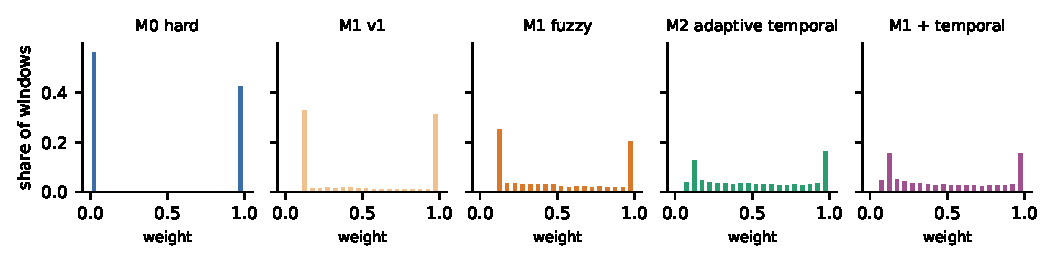
\includegraphics[width=\linewidth]{gate_weights.pdf}
\caption{Distribution of window weights for each gate. M0 is binary (43\% kept). M1 v1 collapses towards 0.1/1.0. M1, M2 and M1\,+\,temporal give graded weights; smoothing moves more weights to intermediate values.}\label{fig:weights}
\end{figure}

\begin{table}[h]
\centering\small
\caption{Gate behaviour on all 23{,}683 windows.}\label{tab:gates}
\begin{tabular}{@{}lcccc@{}}
\toprule
Gate & mean weight & weights at 0.1 or 1 & corr.\ with M0 & corr.\ with M1\\
\midrule
M0 hard & 0.43 & 100\% & 1.00 & 0.28\\
M1 v1 (within trial) & 0.53 & 61\% & 0.81 & 0.33\\
M1 fuzzy & 0.51 & 41\% & 0.28 & 1.00\\
M2 adaptive temporal & 0.53 & 24\% & 0.19 & 0.92\\
M2 adaptive-only & 0.53 & 40\% & 0.31 & 0.94\\
M2 causal & 0.54 & 31\% & 0.24 & 0.92\\
M1\,+\,temporal & 0.51 & 26\% & 0.17 & 0.97\\
\bottomrule
\end{tabular}
\end{table}

\paragraph{Superseded pilot numbers.} A single-participant pilot (35--38\%) and a five-participant run (about 35\%) were shown before these fixes. Defects 2--4 inflated both, because the classifiers mostly predicted the majority class. They should not be cited.

\section{Results}
\begin{table}[h]
\centering\small
\setlength{\tabcolsep}{4.2pt}
\caption{Trial-level accuracy (\%), mean of 3 seeds, 12 participants, 4{,}430 sentences. Chance is 33.3\%. Best value per row in bold. MF1 is macro-F1 averaged over the five bands.}\label{tab:main}
\begin{tabular}{@{}llcccccccc@{}}
\toprule
 & Band & No gate & M0 & M1 & M1 v1 & M2 & M2 adapt. & M2 causal & M1+temp.\\
\midrule
\multirow{7}{*}{5-fold}
 & delta & 32.3 & 32.7 & 33.1 & 32.8 & \textbf{33.7} & 32.8 & 33.2 & 33.3\\
 & theta & 33.2 & 33.0 & \textbf{33.4} & 33.2 & 32.8 & 32.8 & 32.3 & 32.3\\
 & alpha & 33.3 & 33.1 & 33.6 & 33.2 & 33.6 & 33.5 & \textbf{34.2} & 33.9\\
 & beta  & \textbf{34.6} & 33.6 & 33.5 & 32.9 & 34.0 & 34.0 & 34.0 & 34.2\\
 & gamma & 33.1 & 32.8 & 33.1 & \textbf{34.1} & 33.3 & 32.9 & 32.8 & 33.7\\
\cmidrule(l){2-10}
 & mean  & 33.3 & 33.0 & 33.3 & 33.2 & 33.4 & 33.2 & 33.3 & \textbf{33.5}\\
 & MF1   & 31.9 & 32.5 & 32.7 & 32.7 & \textbf{32.8} & 32.4 & 32.2 & 32.2\\
\midrule
\multirow{7}{*}{LOSO}
 & delta & 32.6 & 32.9 & \textbf{33.8} & \textbf{33.8} & 32.4 & \textbf{33.8} & 32.8 & 32.9\\
 & theta & 32.9 & 32.9 & 31.7 & \textbf{33.1} & 31.4 & 32.5 & 32.1 & 32.0\\
 & alpha & 33.1 & 33.8 & 33.5 & 31.9 & 34.6 & 33.7 & \textbf{34.9} & 34.3\\
 & beta  & \textbf{35.2} & 34.2 & 33.4 & 33.5 & 34.0 & 32.9 & 33.6 & 34.8\\
 & gamma & \textbf{34.4} & 34.2 & 33.1 & 34.3 & 32.5 & 33.5 & 33.1 & 32.9\\
\cmidrule(l){2-10}
 & mean  & \textbf{33.7} & 33.6 & 33.1 & 33.3 & 33.0 & 33.3 & 33.3 & 33.4\\
 & MF1   & 32.3 & \textbf{33.3} & 32.9 & 33.0 & 32.6 & 32.9 & 32.2 & 32.9\\
\bottomrule
\end{tabular}
\end{table}

\begin{figure}[h]
\centering
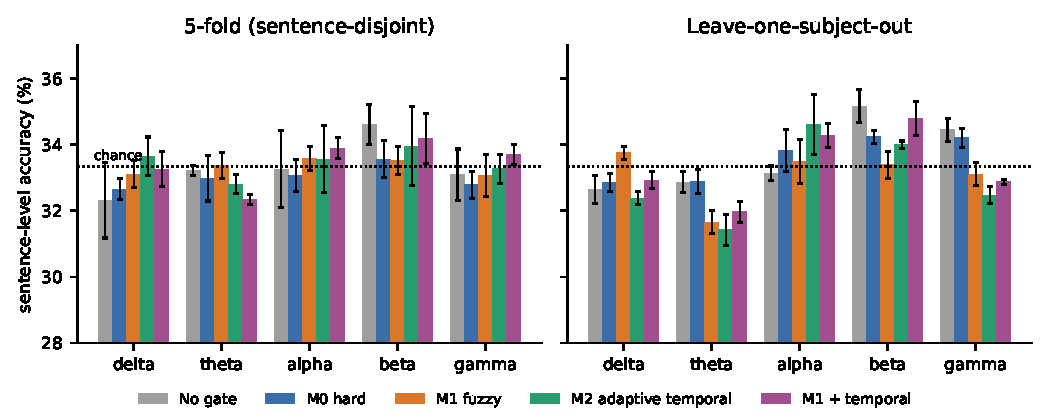
\includegraphics[width=\linewidth]{results_bars.pdf}
\caption{Accuracy per band, protocol and gate (mean $\pm$ SD over 3 seeds). The dotted line is chance (33.3\%). The y-axis starts at 28\%; all differences lie within about 2 points.}\label{fig:bars}
\end{figure}

\begin{table}[h]
\centering\small
\caption{Each proposed gate minus M0, over 15 band$\times$seed runs per protocol. ``Ahead'' counts runs in which the proposed gate beat M0. Participants helped and the Wilcoxon $p$ use per-participant LOSO accuracy averaged over bands and seeds.}\label{tab:delta}
\begin{tabular}{@{}lcccccc@{}}
\toprule
 & \multicolumn{2}{c}{5-fold} & \multicolumn{4}{c}{LOSO}\\
\cmidrule(lr){2-3}\cmidrule(l){4-7}
Model & mean $\Delta$ & ahead & mean $\Delta$ & ahead & participants helped & Wilcoxon $p$\\
\midrule
M1 fuzzy & $+0.32$ & 11/15 & $-0.52$ & 4/15 & 4/12 & 0.15\\
M1 v1 & $+0.22$ & 9/15 & $-0.28$ & 7/15 & 4/12 & 0.38\\
M2 adaptive temporal & $+0.44$ & 10/15 & $-0.62$ & 3/15 & 3/12 & 0.11\\
M2 adaptive-only & $+0.20$ & 10/15 & $-0.33$ & 4/15 & 5/12 & 0.42\\
M2 causal & $+0.25$ & 9/15 & $-0.27$ & 3/15 & 5/12 & 0.47\\
M1\,+\,temporal & $\mathbf{+0.47}$ & \textbf{13/15} & $\mathbf{-0.23}$ & 7/15 & 4/12 & 0.38\\
\bottomrule
\end{tabular}
\end{table}

\begin{figure}[h]
\centering
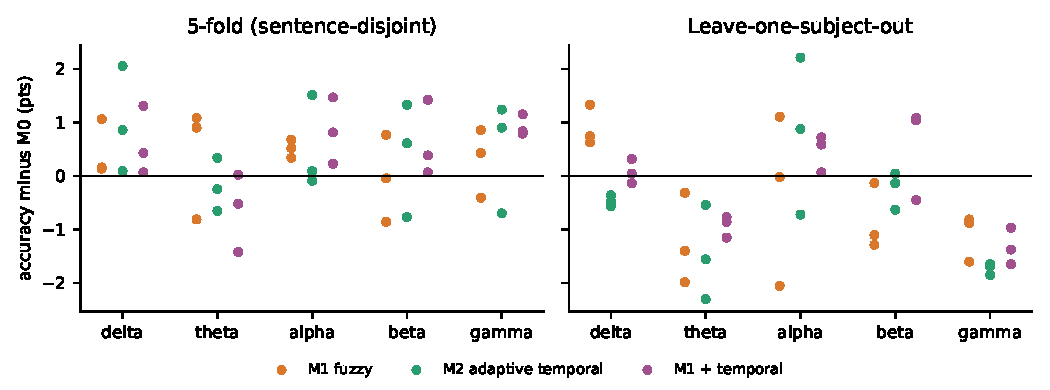
\includegraphics[width=\linewidth]{minus_m0.pdf}
\caption{Accuracy of M1, M2 and M1\,+\,temporal minus M0 for each band and seed. The small gains under 5-fold cross-validation do not carry over to unseen participants (LOSO).}\label{fig:delta}
\end{figure}

\begin{table}[h]
\centering\small
\caption{Reference: L2 logistic regression ($C{=}0.01$, class-balanced) on sentence-mean features. This estimates the accuracy achievable with these features on ZuCo.}\label{tab:ceiling}
\begin{tabular}{@{}lcc@{}}
\toprule
Features & 5-fold & LOSO\\
\midrule
EEG entropies (380 features) & 35.2 & 34.9\\
Eye features (8) & 33.4 & 34.2\\
EEG $+$ eye & 35.2 & 35.5\\
\bottomrule
\end{tabular}
\end{table}

\paragraph{Findings.}
\begin{enumerate}
  \item \textbf{All models are at chance.} The 80 band/protocol/model cells lie between 31.4\% and 35.2\%. Eight are individually above chance (one-sided binomial $p<0.05$), against about four expected by chance alone. They are scattered across models, and neither M0 nor M1 has any.
  \item \textbf{No proposed gate beats M0 reliably.} The proposed gates lead by $+0.2$ to $+0.5$ points under 5-fold cross-validation but trail by $-0.2$ to $-0.6$ points under LOSO (Table~\ref{tab:delta}). No overall difference is significant. The individually significant band-level comparisons favour M0: M1 in theta ($-1.2$\pts, $p_W{=}0.010$) and M2 in gamma ($-1.7$\pts, $p_W{=}0.016$), both LOSO. Neither survives a multiple-comparison correction.
  \item \textbf{M1\,+\,temporal is the most consistent proposed gate.} It leads M0 in 13 of 15 5-fold runs and has the smallest LOSO deficit. Temporal smoothing on M1's fixed gate held up better than M2's per-participant breakpoints, whose weights are nearly identical to M1's ($r{=}0.92$--$0.94$).
  \item \textbf{The classifier works as intended.} All models predict the three classes in roughly their true proportions (e.g.\ M1, LOSO: 34.6/33.0/32.3\% against true shares of 30.8/34.8/34.4\%) and keep 12--14 rules.
  \item \textbf{The features contain almost no sentiment signal.} Even the logistic-regression reference reaches only about 35\% (Table~\ref{tab:ceiling}). A gate can help only if some windows carry more class information than others; on ZuCo, no window carries meaningful information.
\end{enumerate}

\section{Discussion}
\textbf{Why ZuCo cannot discriminate between gates.} (i) The label is the sentiment of the text, not an emotion induced in the reader. Participants read for comprehension, and a review being negative rarely changes how the reader feels. (ii) Sentences last 2--30\,s, compared with minutes-long film clips in SEED-IV, so the affective response is brief and entropy features must be computed on 1-s windows. (iii) The gate assumes that pupil dilation marks emotional arousal. During reading, pupil size is driven mainly by gaze position (the camera sees the pupil at an angle), luminance and reading load, so the gate selects windows for reasons unrelated to emotion. (iv) EEG during reading is dominated by language processing and eye-movement activity, which do not differ by sentiment.

\textbf{What the experiment does show.} The fuzzy gates (M1, M2, M1\,+\,temporal) are drop-in replacements for the hard threshold. They keep every window, avoid a hard cut-off and do not meaningfully reduce performance. The pipeline is now verified end to end on real EEG and eye-tracking data. Eight defects that synthetic data could not reveal were found and fixed, and every model was evaluated without train/test leakage.

\textbf{Limitations.}
\begin{itemize}
  \item A single dataset, and not an emotion dataset.
  \item 19 of 105 channels.
  \item Pupil diameter derived from area.
  \item Gate parameters fixed in advance (not tuned).
  \item Three seeds.
\end{itemize}

\section{Conclusion and next steps}
On real EEG and eye-tracking data (ZuCo~1.0, 12 participants, 4{,}430 sentences), the proposed fuzzy (M1), adaptive temporal (M2) and combined (M1\,+\,temporal) eye gates perform on par with the paper's hard gate (M0). They gain at most 0.5 points under 5-fold cross-validation, lose at most 0.6 points on unseen participants, and no difference is significant. Because no model, including a strong non-fuzzy reference, exceeds about 35\% on this text-sentiment task, ZuCo cannot discriminate between gating strategies. Next steps:
\begin{enumerate}
  \item Obtain the SEED-IV (or MAHNOB-HCI) licence and rerun the identical pipeline with the paper's 4-s windows, $m{=}5,\tau{=}2$ and 62 channels. This is the actual test of M1, M2 and M1\,+\,temporal.
  \item Optionally, test the gates on a ZuCo target that EEG and eye tracking do encode, such as normal versus task-specific reading (ZuCo tasks 2 and 3).
  \item Fix any tuning of gate parameters in advance and carry it out by nested cross-validation on training folds only.
\end{enumerate}

\appendix
\section{Reproducibility}
\begin{small}
\begin{verbatim}
python scripts/download_zuco.py --out data/zuco --jobs 6        # ~20 min, 5.97 GB
python -m gfer.zuco --src data/zuco --out data/zuco_npz          # ~2 min
python -m gfer.compare --datasets data/zuco_npz --protocols trial,loso --seeds 0,1,2 \
   --variants none,hard,fuzzy,fuzzy_trialnorm --out results/zuco_final_m0m1
python -m gfer.compare ... --variants adaptive,adaptive_nosmooth,adaptive_causal \
   --out results/zuco_m2/m2_only
python -m gfer.compare ... --variants fuzzy_smooth --out results/zuco_combo/combo_only
python manuscript/zuco_report/make_figures.py                    # figures + stats.json
\end{verbatim}
\end{small}
Raw predictions for every sentence, fold, band, seed and model are stored in \texttt{raw.json} in each results folder. Every number in this report is in \texttt{manuscript/zuco\_report/stats.json}. The ZuCo-specific settings are recorded in \texttt{data/zuco\_npz/meta.json}. Each comparison run takes about 1--1.5\,h on 8 cores (3--4$\times$ longer on a laptop in low-power mode). Code: \texttt{gfer/zuco.py} (loader), \texttt{gfer/gates.py} (M0, M1), \texttt{gfer/adaptive\_gate.py} (M2 and smoothing), \texttt{gfer/compare.py} (experiments). The unit tests are in \texttt{tests/test\_gates\_zuco.py}.

\section*{References}
\begin{small}
\begin{itemize}
  \item J.~Farhadi Sedehi, N.~Jafarnia Dabanloo, K.~Maghooli, A.~Sheikhani, ``Recognition of emotional categories using mined fuzzy rules from electroencephalogram signals with gated eye track data approach,'' \emph{IEEE Access}, 12:118122--118140, 2024. doi:10.1109/ACCESS.2024.3430934.
  \item N.~Hollenstein, J.~Rotsztejn, M.~Troendle, A.~Pedroni, C.~Zhang, N.~Langer, ``ZuCo, a simultaneous EEG and eye-tracking resource for natural sentence reading,'' \emph{Scientific Data}, 5:180291, 2018. doi:10.1038/sdata.2018.291.
  \item W.-L.~Zheng, W.~Liu, Y.~Lu, B.-L.~Lu, A.~Cichocki, ``EmotionMeter: a multimodal framework for recognizing human emotions,'' \emph{IEEE Trans.\ Cybernetics}, 49(3):1110--1122, 2019 (SEED-IV). doi:10.1109/TCYB.2018.2797176.
\end{itemize}
\end{small}
\end{document}
